\section{Hashlife}
\subsection{un peu d'histoire}
\begin{figure}[htp]
        \center
        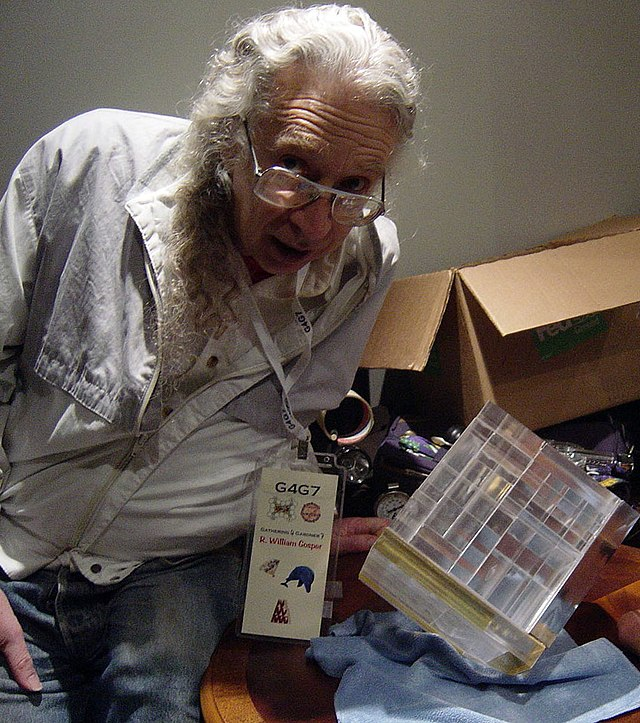
\includegraphics[scale=0.2]{images/imgHashlife/Bill_Gosper_2006.jpg}
        \caption{William (aussi appelé Bill) Gosper l'inventeur de Hashlife}
\end{figure}

Hashlife fut initialement développé en 1984 par le mathématicien William Gosper qui avait pour but d'optimiser la résolution de formes Régulières dans les automates cellulaires, notamment le jeu de la vie de John Conway. A l'époque les mathématiciens et les informaticiens essayaient de développer leur propre algorithme pour optimiser le jeu de la vie. Parmi les méthodes d'optimisations communes, on trouve par exemple l'utilisation complète des registres afin d'économiser de l'espace. Il est aussi possible de reconnaître les oscillateurs et de les pré-calculer pour ne pas avoir à les prendre en compte dans le calcul complet. Cependant, ces optimisations devenaient lourdes et fournissaient des résultats moins intéressants.

En essayant de simplifier les choses, William Gosper crée alors l'algorithme Hashlife. Il publie donc \textit{"Exploiting Regularities in Large Cellular Spaces"}, un article détaillant son algorithme.

Toutefois, étant donné la complexité de l'algorithme, aucune implémentation ne sera créée directement après la publication de cet article, ce qui le cachera initialement du grand public et retardera son implémentation. Hashlife devient alors la source de rumeurs pendant les années 80 lorsque Rudy Rucker déclara avoir été témoin de simulations impressionnantes du jeu de la
vie, lors d'une visite chez William Gosper. 

Épaté, il dira bien plus tard : 

\textit{"Gosper showed me some incredible game of life simulations that were based on a weird speed-up algorithm of his, called 'Hashlife'. I remember him sharing the source code for the trick, but for me that was strictly a case of the Mathematician Godfather: He makes you an offer you can't understand"}

Plusieurs années plus tard, en 2005, sort GOLLY l'une des premières implémentations de Hashlife, ainsi que de Quicklife. Cette implémentation deviendra rapidement la référence dans le monde du jeu de la vie. Elle permet en effet de simuler des univers du jeu de la vie absolument gigantesques - grâce à des optimisations de mémoire - à des vitesses hallucinantes. En effet, GOLLY utilise Quicklife dans les cas ou Hashlife est trop lent. L'intérêt du public pour ce logiciel est sans précédent et permet de populariser le jeu de la vie.

\subsection{Aperçu}
Comme dit précédemment, Hashlife est un algorithme utilisé pour optimiser les formes de vie régulières dans le jeu de la vie. Cependant, grâce à l'augmentation de la taille de la mémoire de nos ordinateurs, l'algorithme est plus généraliste. Il peut optimiser plus de conditions, et il n'est donc plus très pertinent de développer une solution hybride pour un projet simple.

Mais qu'optimise Hashlife?

Dans le jeu de la vie classique, il existe deux grandes limitations :
\begin{itemize}
\item{La vitesse}
\item{La taille}
\end{itemize}
William Gosper décide donc d'orienter son attention vers ces limitations.

Pour régler le problème de la taille de la simulation, on change de structure de données. C'est à dire que l'on utilise un quadtree sur lequel on effectue une génération du jeu de la vie sans décompresser le quadtree.

Pour optimiser la vitesse, on mémoize les nodes déjà utilisées afin de les réutiliser quand on en a besoin.

Pour aller plus loin, on utilise ce que Gosper appelle la "superspeed", cette partie de l'algorithme qui est responsable du gain de vitesse phénoménal de Hashlife.

\subsection{Compression de l'espace}
\subsubsection{QuadLife}

La base de Hashlife réside dans l'utilisation de quadtrees pour stocker les cellules de notre univers. Un quadtree, aussi appelé "arbre quaternaire" dans le pays des baguettes, est une structure de données arborescente représentée de cette manière : 

\begin{figure}[htp]
        \center
        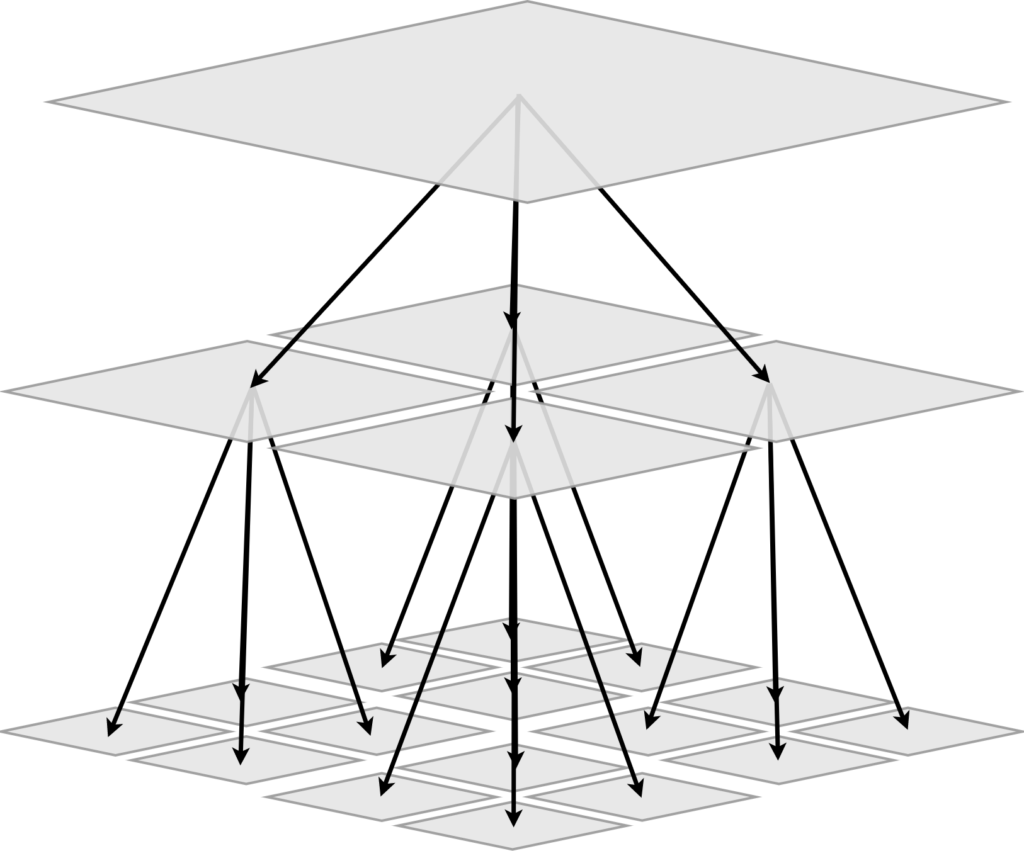
\includegraphics[scale=0.1]{images/imgHashlife/representationquadtree.png}
        \caption{représentation simple d'un quadtree}
\end{figure}

Elle est plus communément utilisée dans la compression de couleurs pour les images, mais cette structure de données a bien d'autres applications, l'une d'entre elle étant évidemment Hashlife!

\begin{figure}[htp]
        \center
        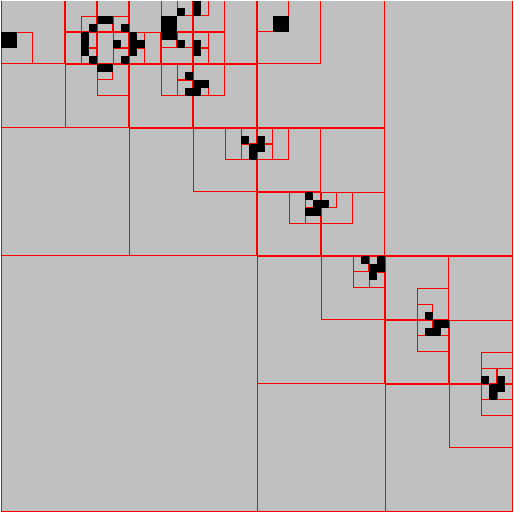
\includegraphics[scale=0.2]{images/imgHashlife/quadLife1.png}
        \caption{utilisation de Quadtree pour stocker un pistolet à Gliders dans notre projet}
\end{figure}

Rajouter des cellules vivantes à un quadtree est en réalité assez simple.
Il faut juste avoir défini au préalable la taille de notre univers (forcément en puissance de 2 car un quadtree ne peut que représenter des puissances de 2) puis utiliser une fonction récursive pour traverser le quadtree jusqu'à atteindre le niveau 0 et mettre la case à la valeur désirée. On peut aussi obtenir la valeur d'une cellule spécifique exactement de la même manière. On peut donc, si on le veut, implémenter le jeu de la vie de cette manière, mais cela serait extrêmement inefficace et empirerait notre problème de vitesse ainsi que de taille car on aurait alors décompressé notre quadtree.

Il nous faut donc une routine qui effectue le jeu de la vie directement sur un quadtree sans rien décompresser. Cette partie est très complexe mais je vais faire de mon mieux pour essayer de simplifier sans perdre des information clés.

On veut faire une fonction dans laquelle on met un Quadtree en argument et la fonction nous renvoie le Quadtree de prochaine génération qu'on peut en déduire.

Premier problème: on ne peut pas déduire la valeur de toutes les cases du quadtree car celles qui sont collées à la bordure ont des voisins impossibles à déduire car externes à la node concernée. Il faudrait prendre la node parent pour trouver les voisins dans les nodes adjacentes, mais il faudrait alors prendre tout le quadtree (car la node parent a aussi des nodes adjacentes) donc ce n'est pas une solution viable.

\begin{figure}[htp]
        \center
        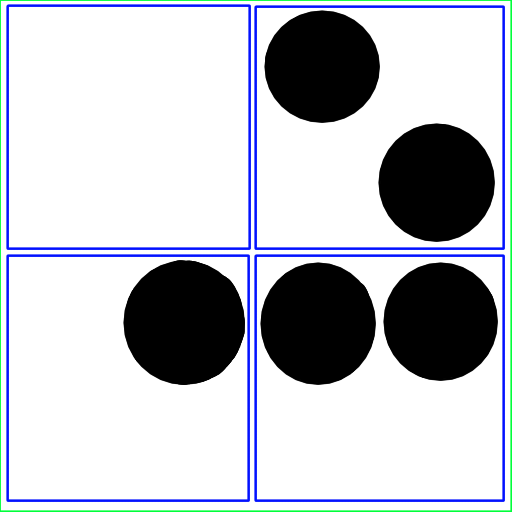
\includegraphics[scale=0.7]{images/imgHashlife/GOLfig1.png}
        \caption{on ne peut pas vérifier tout les voisins des cellules depuis les arbres bleus }
\end{figure}

A la place nous allons nous contenter de renvoyer la node centrale de notre quadtree, c'est ce qui va nous permettre d'éviter de décompresser le quadtree. Essentiellement, nous ne pouvons être sûrs de calculer que les nodes qui ont des voisins dans notre quadtree, nous ne calculons que la node centrale pour laisser les enfants de notre quadtree faire le reste du boulot car la fonction est récursive.

Notre fonction prend donc un quadtree en entrée et renvoie la node centrale de celui-ci à la prochaine génération. Il peut donc sembler correct d'appliquer la fonction sur chaque node mais cela laisserait des "trous" non calculés dans notre quadtree, la fonction ne fonctionne toujours pas complètement...

\begin{figure}[htp]
        \center
        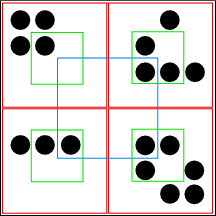
\includegraphics[scale=0.7]{images/imgHashlife/GOLfig2.png}
        \caption{voici pourquoi on ne peut pas simplement renvoyer la node centrale de chaque node. Beaucoup d'espace reste non-calculé et la node centrale initiale n'est pas complètement calculée }
\end{figure}

Notre fonction est cependant "correcte" pour un cas spécifique de notre calcul. Si notre node est juste au-dessus du niveau cellulaire, on peux l'adapter pour calculer directement les quatre cellules qui sont centrales à cet arbre de manière très similaire au jeu de la vie de base. Cette étape est appelé le calcul lent.

On lui crée donc sa propre fonction "calculLent()" qui prend un quadtree de niveau 2 et renvoie un arbre de niveau 1 à la prochaine génération. Notre objectif est à présent d'appeler calcul lent dans toutes les nodes qui arrivent au niveau cellulaire.

\begin{figure}[htp]
        \center
        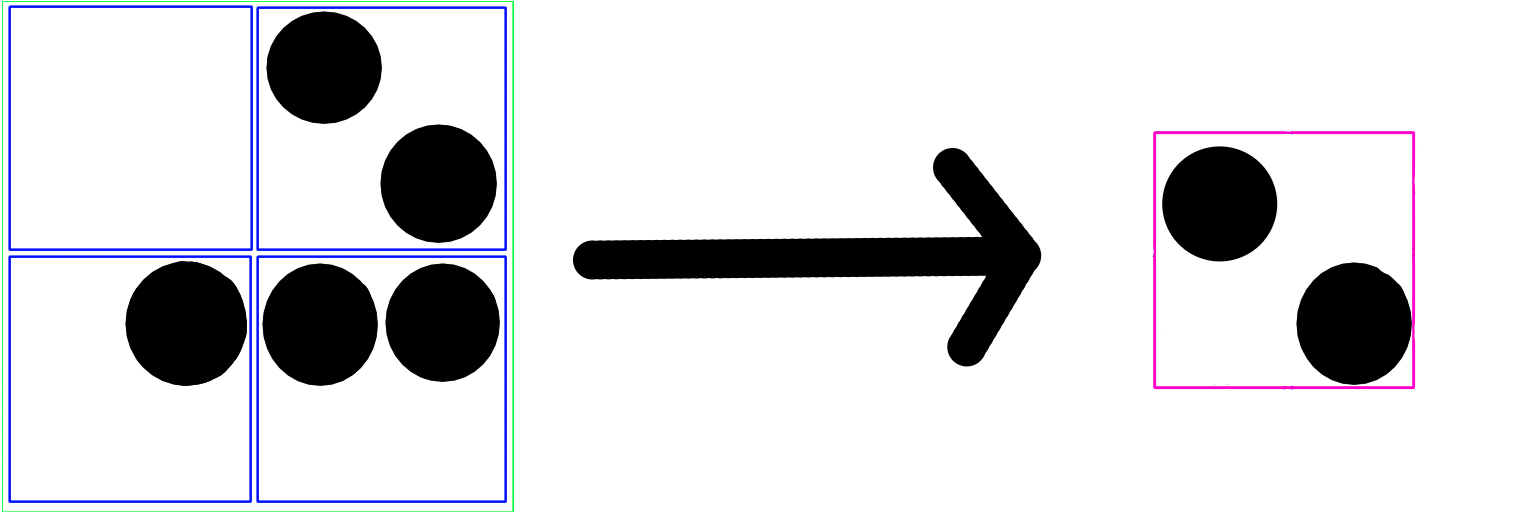
\includegraphics[scale=0.4]{images/imgHashlife/GOLfig3.png}
        \caption{l'arbre violet est le résultat obtenu en appliquant "calculLent()" sur l'arbre vert}
\end{figure}

Pour ce faire, on doit vérifier chaque node non-vide ce qui n'équivaut \textbf{pas} à décompresser le quadtree, vu qu'on ne vérifie pas chaque cellule et qu'on saute les grands espaces vides lorsqu'il y en a.

C'est là que vient la solution de génie: Prenons une node de niveau 3 pour laquelle on veut calculer la prochaine génération de sa node centrale.

Pour ce faire, nous allons générer 9 nodes intermédiaires de niveau 1, puis les rassembler en groupe de 4 pour obtenir des nodes de niveau 2 sur lesquelles on peut utiliser "calculLent()" pour assembler la node centrale de notre node. Rappelez-vous: notre fonction renvoie un arbre deux fois plus petit! Ainsi on a effectué notre prochaine génération sur un arbre de niveau 3. 

\begin{figure}[htp]
        \center
        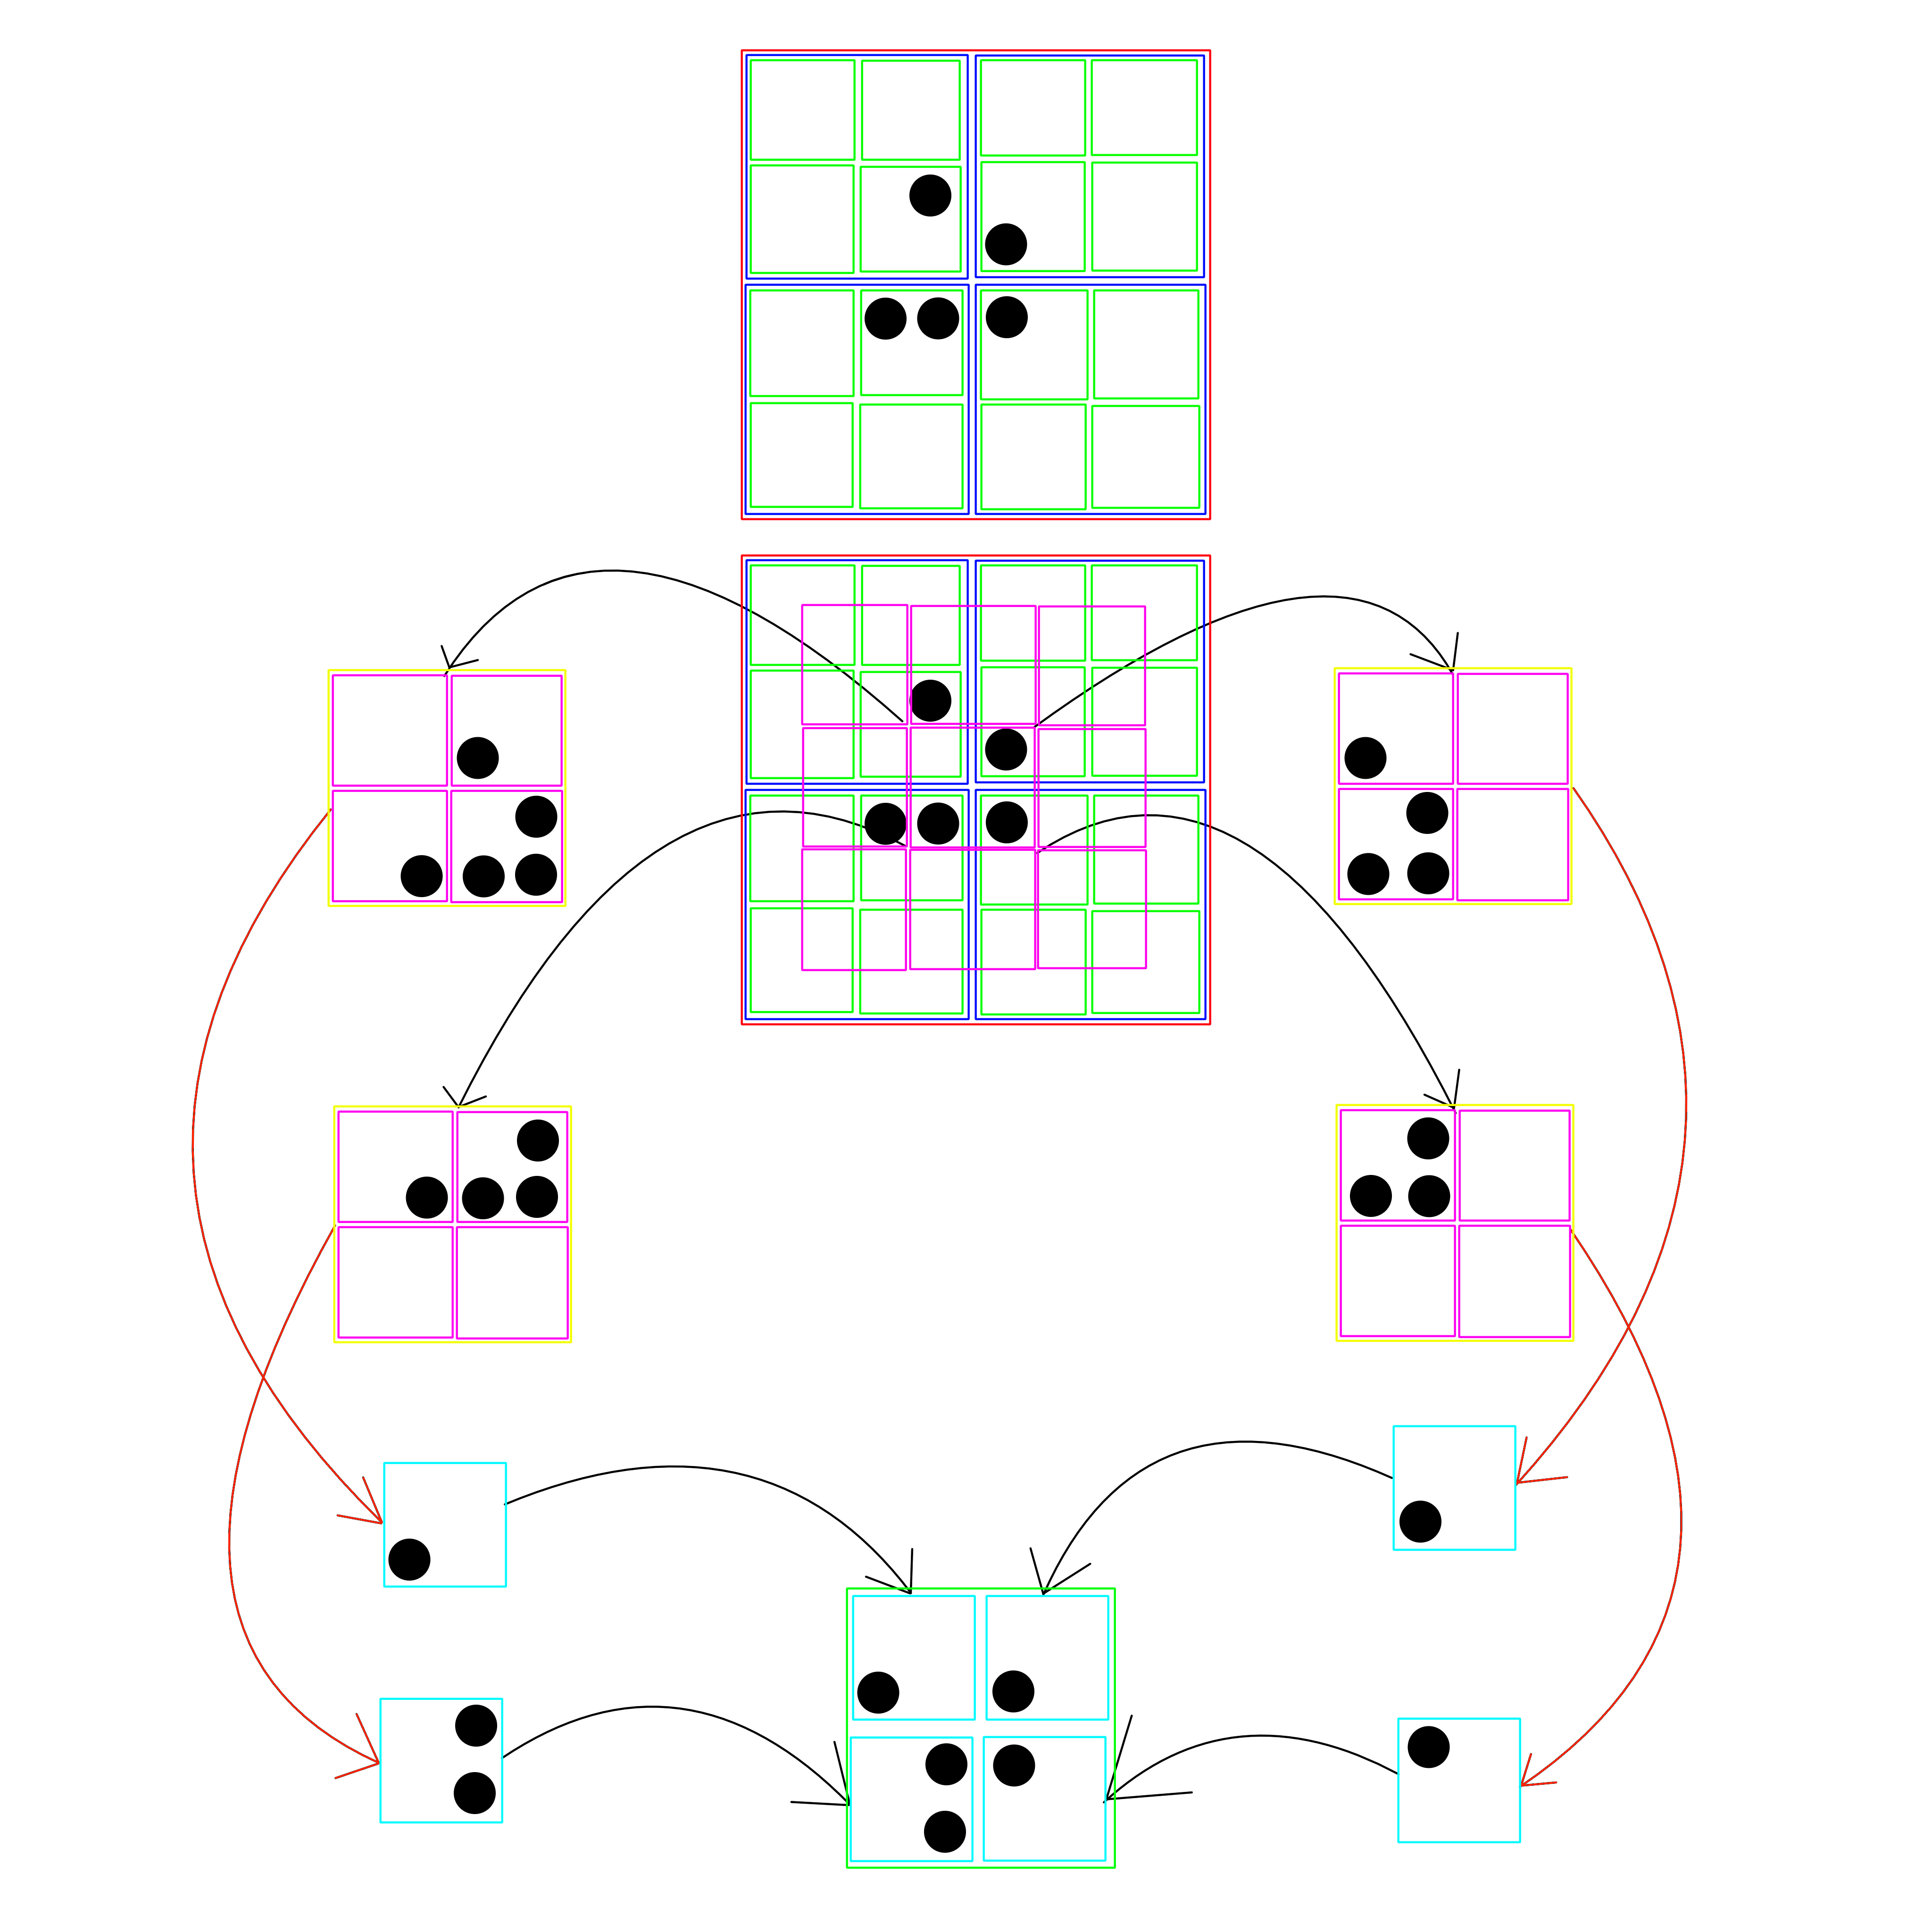
\includegraphics[scale=0.225]{images/imgHashlife/nextGen.png}
        \caption{on groupe les 9 nodes en groupes de 4 sur lesquelles on appelle nextGen (flèches rouges), on assemble le résultat, ce qui nous donne la node centrale une génération en avant de l'arbre initial}
\end{figure}

Chouette! Mais devons-nous répéter l'opération pour chaque node? Heureusement non! Si on met juste une condition pour vérifier si le niveau est égal à 2, alors: si oui, on fait "calculLent()", sinon on fait l'algorithme décrit précédemment. Appelons notre fonction "nextgen()".

\SetKwComment{Comment}{/* }{ */}
\begin{algorithm}
\tiny
\caption{nextgen()}\label{alg:nextgen}
\eIf{level = 2}{
    calculLent()\;
}{
    \Comment{on génère les 9 nodes}
    node1$\gets$ CréerNodeAuxiliaire\_1\;
    node2$\gets$ CréerNodeAuxiliaire\_2\;
    node3$\gets$ CréerNodeAuxiliaire\_3\;
    node4$\gets$ CréerNodeAuxiliaire\_4\;
    node5$\gets$ CréerNodeAuxiliaire\_5\;
    node6$\gets$ CréerNodeAuxiliaire\_6\;
    node7$\gets$ CréerNodeAuxiliaire\_7\;
    node8$\gets$ CréerNodeAuxiliaire\_8\;
    node9$\gets$ CréerNodeAuxiliaire\_9\;
    \Comment{on assemble les 9 nodes en 4 nodes}
    \Comment{on appelle récursivement l'algorithme afin d'obtenir la node centrale}
    \Comment{des 4 nodes à la prochaine génération}
    tmpNode1$\gets$ assembleNode(node1, node2, node4, node5).nextGeneration()\;
    tmpNode2$\gets$ assembleNode(node2, node3, node5, node6).nextGeneration()\;
    tmpNode3$\gets$ assembleNode(node4, node5, node7, node8).nextGeneration()\;
    tmpNode4$\gets$ assembleNode(node5, node6, node8, node9).nextGeneration()\;
    \Comment{on assemble les 4 nodes et on renvoie le résultat}
    resultat$\gets$ assemblerNode( tmpNode1,tmpNode2,tmpNode3,tmpNode4 )\;
}
\end{algorithm}


A ce stade, la partie difficile de cette partie est terminée, mais nous n'avons pas encore fini, en effet si notre algorithme diminue la taille de notre node par 2 à chaque génération, nous n'allons pas pouvoir simuler tout notre quadtree et il rétrécira au fur et à mesure des générations.

La solution est très simple : créer un arbre "bordure" dont la node centrale est l'arbre sur lequel on veut passer à la prochaine génération. Le reste de ses nodes est vide. On appellera cette fonction "extend()".

\begin{figure}[htp]
        \center
        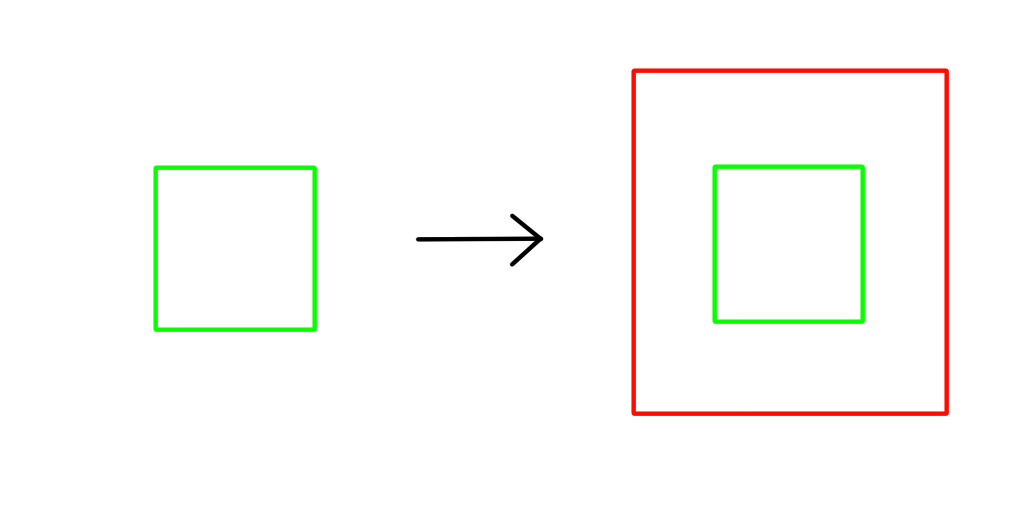
\includegraphics[scale=0.5]{images/imgHashlife/extend.png}
        \caption{l'arbre vert est l'arbre initial, l'arbre rouge est l'arbre bordure, \textit{extend} retourne l'arbre bordure}
\end{figure}

Maintenant il ne nous reste plus qu'à assembler nos fonctions pour créer "fullnextgen()"

Dans un premier temps, on utilise "extend", puis on appelle "nextGen()" et on retourne le résultat. Nous avons maintenant calculé une génération du jeu de la vie dans un quadtree, ce qui n'est pas particulièrement rapide (même plus lent qu'un algorithme classique), de plus l'arbre actuel n'est pas hashable, il faut donc le modifier. Nous n'avons pourtant pas travaillé en vain, notre algorithme permet d'avoir un univers "infini" tant que la population de celui-ci n'est pas trop grosse ce qui résout le premier problème du Jeu de la Vie.

\subsubsection{Canonicalisation du Quadtree}
J'ai mentionné dans la partie précédente que notre arbre n'était pas hashable, en effet, pour obtenir ce statut nous allons devoir procéder à la canonicalisation de notre quadtree.

Qu'est-ce que la canonicalisation d'un quadtree?

En termes simples, "Canonicaliser un arbre" revient à rassembler ses nodes similaires en blocs Canoniques. Ainsi, si une forme est trouvée de multiples fois dans l'arbre, nous ne la stockons qu'une seule fois et nous en passons la référence là ou elle est nécessaire. L'intérêt primordial est de réduire la consommation de mémoire, mais dans le cas de Hashlife cela nous permet d'implémenter la mémoization de manière efficace.

\begin{figure}[H]
        \center
        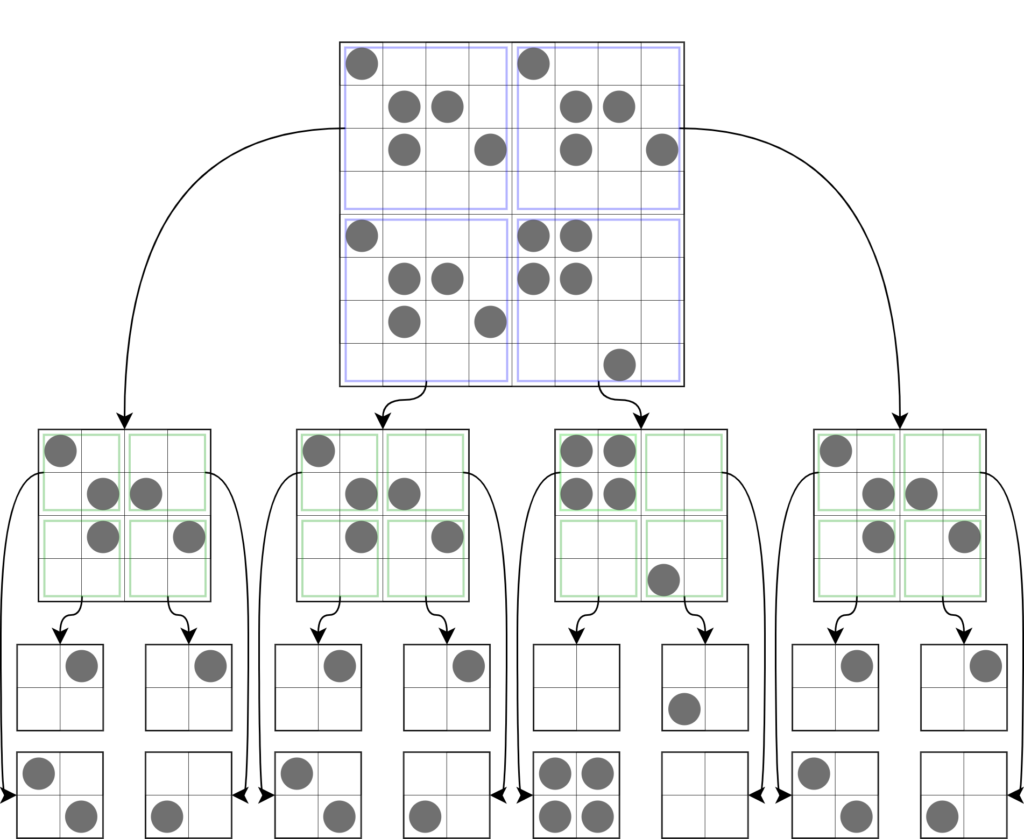
\includegraphics[scale=0.16]{images/imgHashlife/quadtreeNONcanonique.png}
        \caption{voici la représentation de notre arbre actuel, certaines nodes sont identiques et devraient être regroupées!}
\end{figure}

Mais alors, comment allons-nous canoniser notre Quadtree? En théorie c'est en réalité très simple. En effet, il suffit de stocker notre node dans une hashmap avec elle-même comme objet, ainsi quand une node a exactement les mêmes enfants et la même valeur, on peut considérer que les deux objets sont égaux. On peut alors supprimer le nouvel objet et renvoyer la node déjà stockée dans la hashmap. On peut appeler cette fonction "canonicaliser()" ou encore "integre()". Étant donné quelle est moins verbeuse je vais choisir la deuxième option. Finalement, on modifie le constructeur des nodes canoniques afin de les canoniser lors de leur création, on a juste à intégrer la node résultante de la création.

Si on appelle systématiquement le constructeur des nodes canoniques pour créer nos nodes, notre quadtree se canonisera tout seul.

\begin{figure}[H]
        \center
        \includegraphics[scale=0.16]{images/imgHashlife/quadtreecanonique.png}
        \caption{voici la représentation de notre arbre canonisé, les nodes identiques on été regroupées!}
\end{figure}

Même si nous gérons mieux notre mémoire, notre jeu de la vie reste lent. Heureusement, cette étape est la fondation de la partie à suivre qui nous permettra enfin d'aller plus vite qu'une implémentassions classique du jeu de la vie. Il est aussi intéressant de noter que les espaces de forte densité prennent beaucoup moins d'espace que précédemment si ils sont réguliers. Ainsi, nous avons quasiment totalement fait abstraction de la notion d'espace du jeu de la vie.

\subsection{Compression du temps}
\subsubsection{Memoization: Almost-Hashlife}
Maintenant que notre quadtree est canonisé il est trivial d'implémenter la Mémoisation il suffit simplement de rajouter une node appelée next dans notre structure de node, on l'initialisera a null avec le constructeur, cependant on ne prendra pas ce nouveau membre en compte lors de la canonicalisation.
il ne suffit plus que de modifier la fonction "nextGen()" pour vérifier si next est null, si ce n'est pas le cas, on fait le calcul comme précédemment et on initialise next a la valeur du résultat, en revanche si next n'est pas null (et a donc déjà été calculé) on renvoie simplement next.

\begin{algorithm}
\tiny
\caption{nouvelle définition de nextGeneration()}\label{alg:two}
\eIf{next = null}
{
    \Comment{si la node n'est pas calculé on la calcule ici}
    next $\gets$ calculLent()\;
}

\Comment{on renvoie la node précalculée}
resultat $\gets$ next\;
\normalsize
\end{algorithm}

Ainsi on ne refait pas le même calcul deux fois, et après quelques générations énormément de nodes ont été mémoisées, a ce stade l'ordinateur n'effectue quasiment que des lectures dans une hashmap ce qui est très rapide, et ainsi la vitesse d'exécution explose, on est capable de simuler des centaines de génération en une secondes, de plus si le pattern simulé est régulier, il est possible que l'arbre entier soit mémoisé totalement, a ce stade la simulation deviens stable et on n'utilise plus du tout "calculLent()" ce qui va nous permettre de simuler des dizaines de milliers de générations en une seconde, ce qui est vraiment incroyable, mais vu que la simulation n'évolue plus, un peu ennuyant...

On a maintenant un algorithme extrêmement rapide, probablement bien plus rapide que tout autre implémentation du jeu de la vie, même quicklife ne peut pas nous rattraper en nombre de génération par secondes, on pourrait s'arrêter là si on le voulait, la vitesse est suffisante pour simuler des patterns comme le triangle de Sierpinski a des échelles remarquables. Il est a noter que la vitesse est suffisante, nous voulons aller au delà, et c'est ce que va nous permettre Hashlife.
\subsubsection{Superspeed: Hashlife}
Almost-Hashlife nous permet de calculer génération par génération  le jeu de la vie dans un espace quasi-infini, le temps de calcul entre deux génération est le plus petit possible et ne peut être réduit que grâce a des optimisations de bas niveaux comme l'utilisation complète et efficace des registre, du parallélisme SIMD ou du multithreading "simple". Mais d'un point de vue purement algorithmique nous avons atteint le temps de calcul minimal. Mais alors comment accélérer encore plus la simulation? la solution est en réalité plutôt simple : calculer plus de générations pour chaque appel de nextGen(). Pour bien illustrer l'optimisation que nous allons implémenter nous devons revenir a l'implémentation de Quadlife que nous avons abordé précédemment:

Pour passer a la prochaine génération nous générons neufs nodes intermédiaires que nous assemblons pour former quatre nodes sur lesquelles on appelle nextGen() récursivement afin de passer a la prochaine génération Comme montré dans la figure 7.

Pour un arbre de niveau 3 nos 9 nodes temporaires sont de niveau 3-2 = 1, cela ne doit pas changer, cependant, nous allons changer d'approche pour les générer, a la place d'aller chercher  individuellement les 4 nodes nécessaires pour la fabrication de chacune des 9 nodes temporaires individuelles, nous allons prendre des arbres un niveau plus haut ainsi la node temporaire centrale sera la node centrale de l'arbre sur lequel on a appelé nextGen qui est dans notre exemple de niveau 3-1 = 2 les nodes temporaires nw , ne , sw et se sont simplement les enfants correspondants de notre arbre initial, les nodes n, s , w et e sont des mélanges entre les nodes diagonales ex : le bas de nw et le haut de sw combiné donne w.
\begin{figure}[H]
        \center
        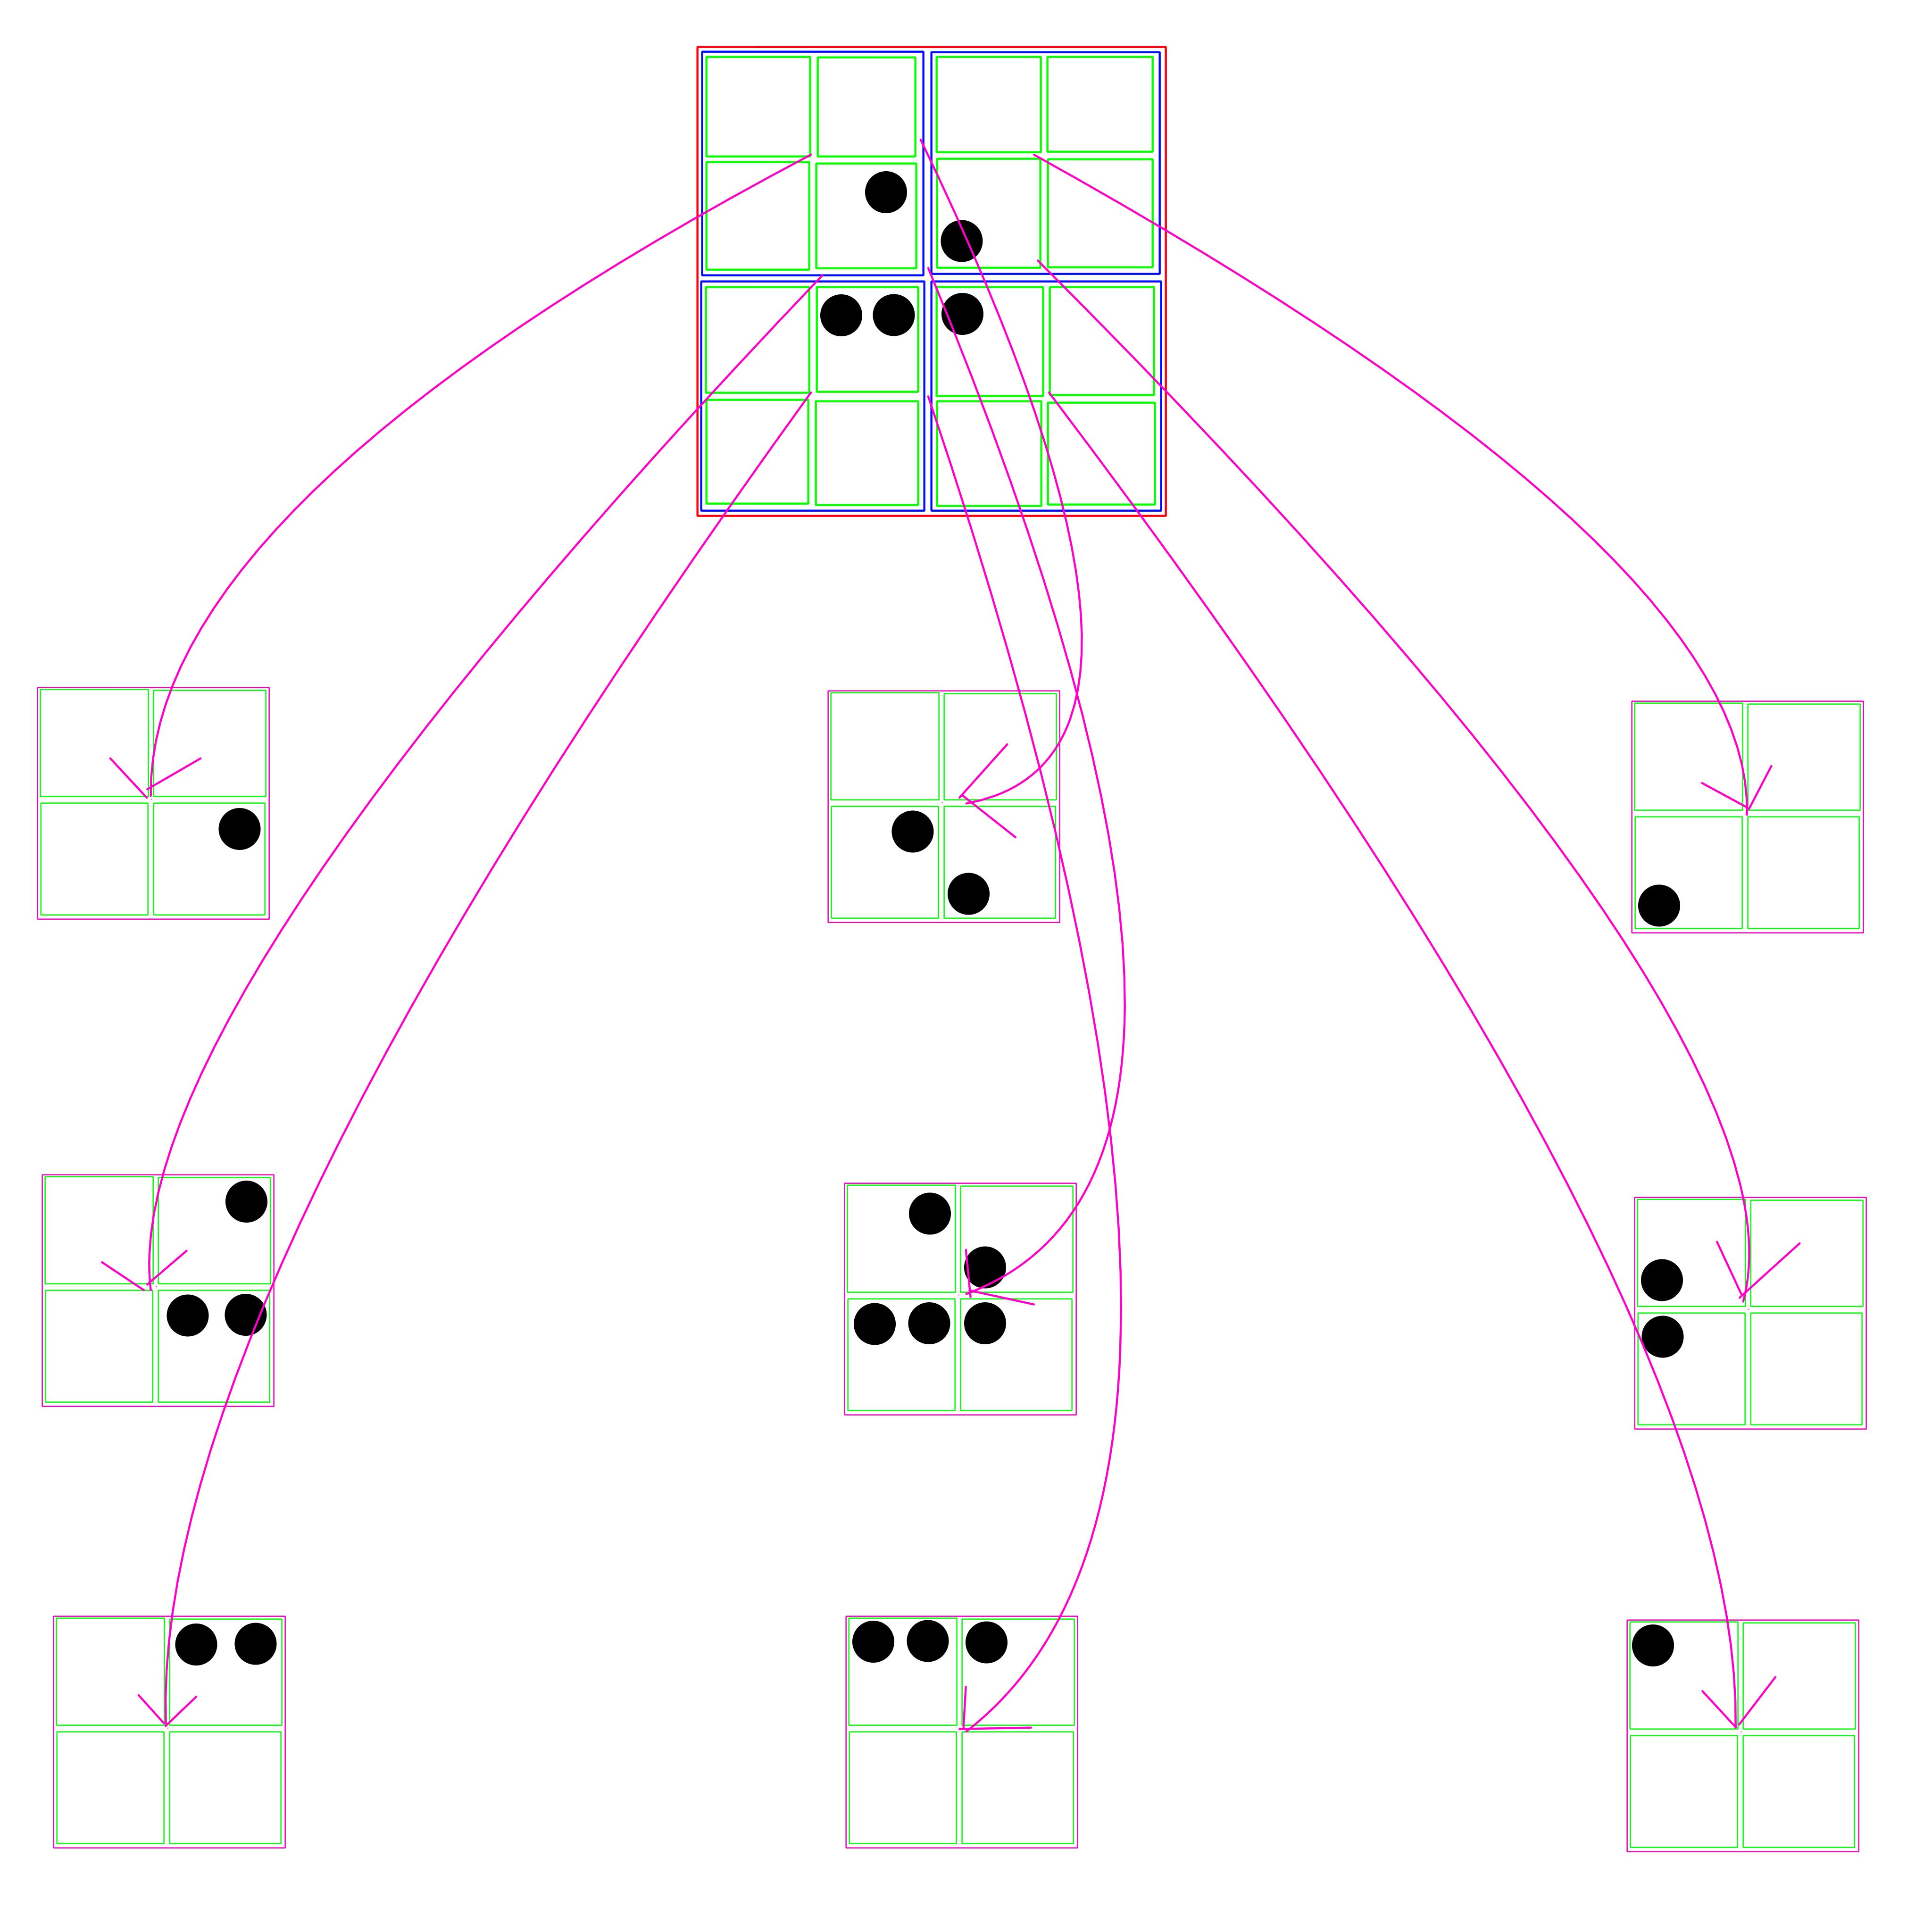
\includegraphics[scale=0.1]{images/imgHashlife/HashlifeStep1.png}
        \caption{Première étape de l'algorithme de Hashlife}
\end{figure}
Ces nouvelles nodes temporaires sont de niveau 2 comme dit précédemment, il faut que nous retrouvons nos nodes de niveau 1, pour les retrouver on pourrait prendre leur node centrale, mais on n'aurais rien fait de très intéressant, a la place nous allons utiliser nextGen pour trouver leur node centrale une génération en avant puis les assembler en nos 4 nodes.
\begin{figure}[H]
        \center
        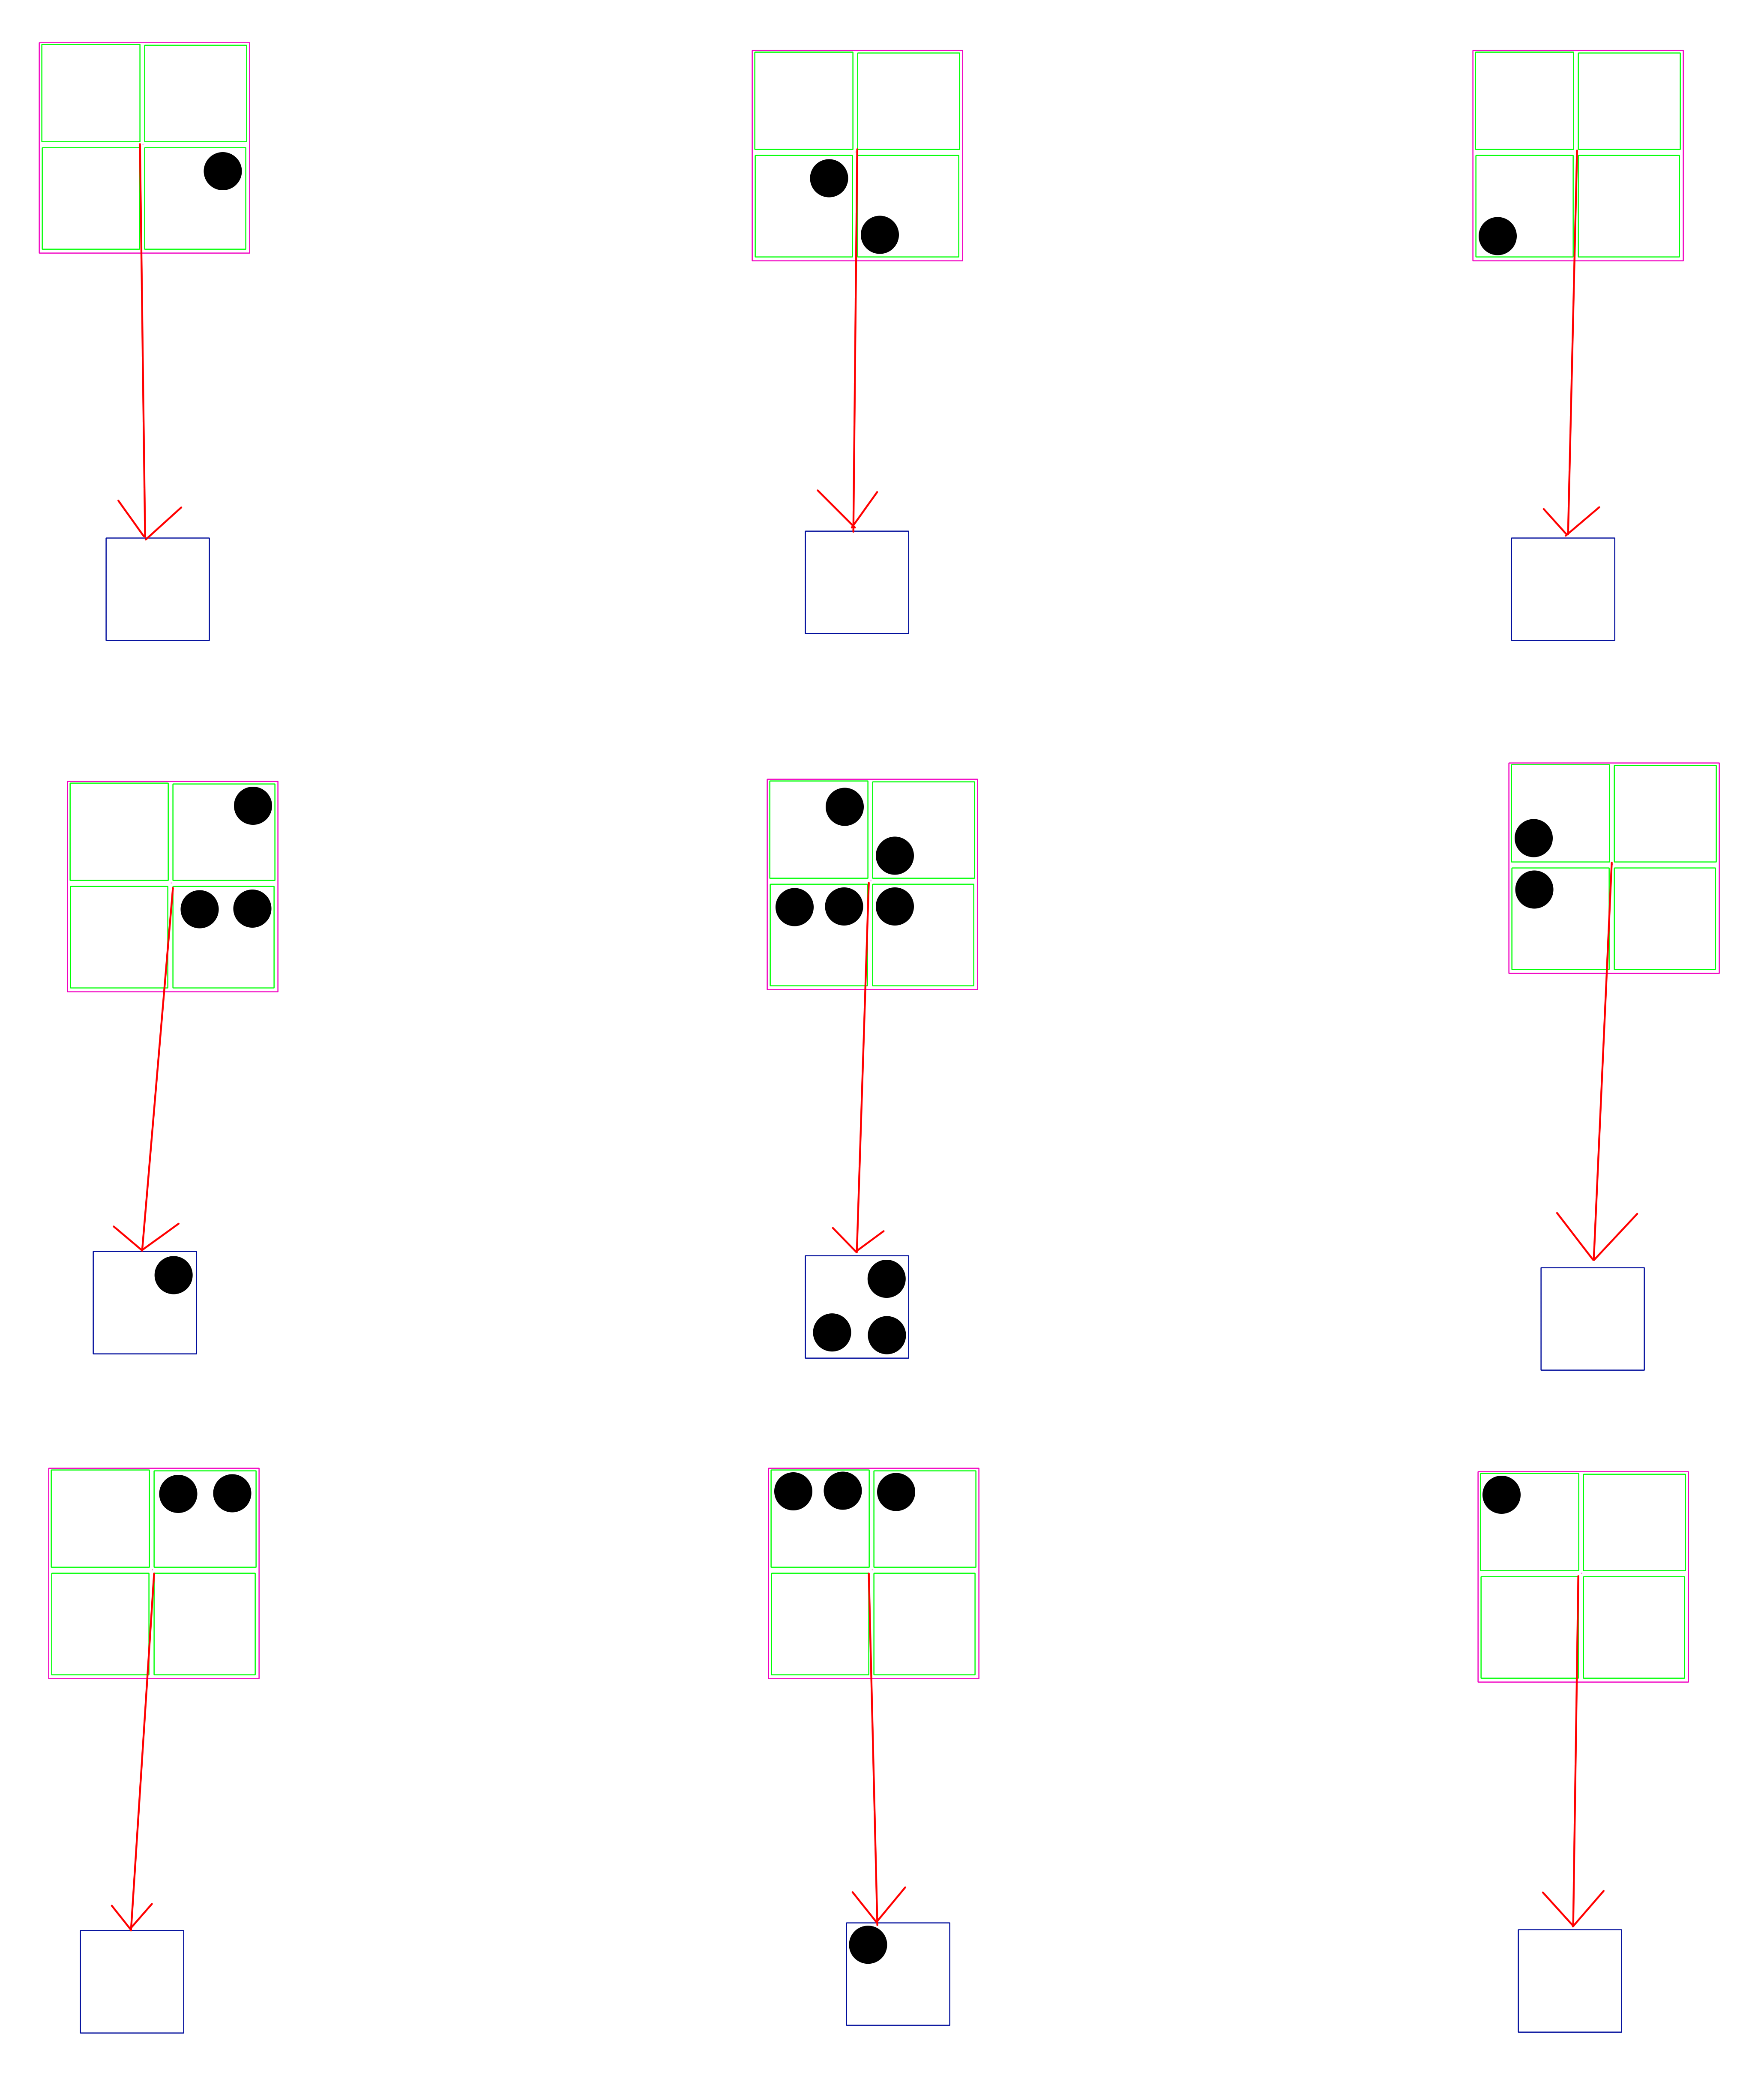
\includegraphics[scale=0.1]{images/imgHashlife/HashlifeStep2.png}
        \caption{Deuxième étape de l'algorithme de Hashlife}
\end{figure}
Nous pouvons alors réutiliser nextGen dessus comme "d'habitude" afin de trouver notre node évoluée cette fois ci non pas d'une génération mais de 2 générations! si on applique l'algorithme sur un niveau plus haut (4) on remarque que l'on ne fait pas 2 mais 4 génération en un seul appel! Et la tendance continue, pour un arbre de niveau 8 on fait 64 générations! Si vous avez l'oeil vous remarquerez que c'est une croissance exponentielle d'écrite par l'équation nbGen = $2^{niveau-2}$.
\begin{figure}[H]
        \center
        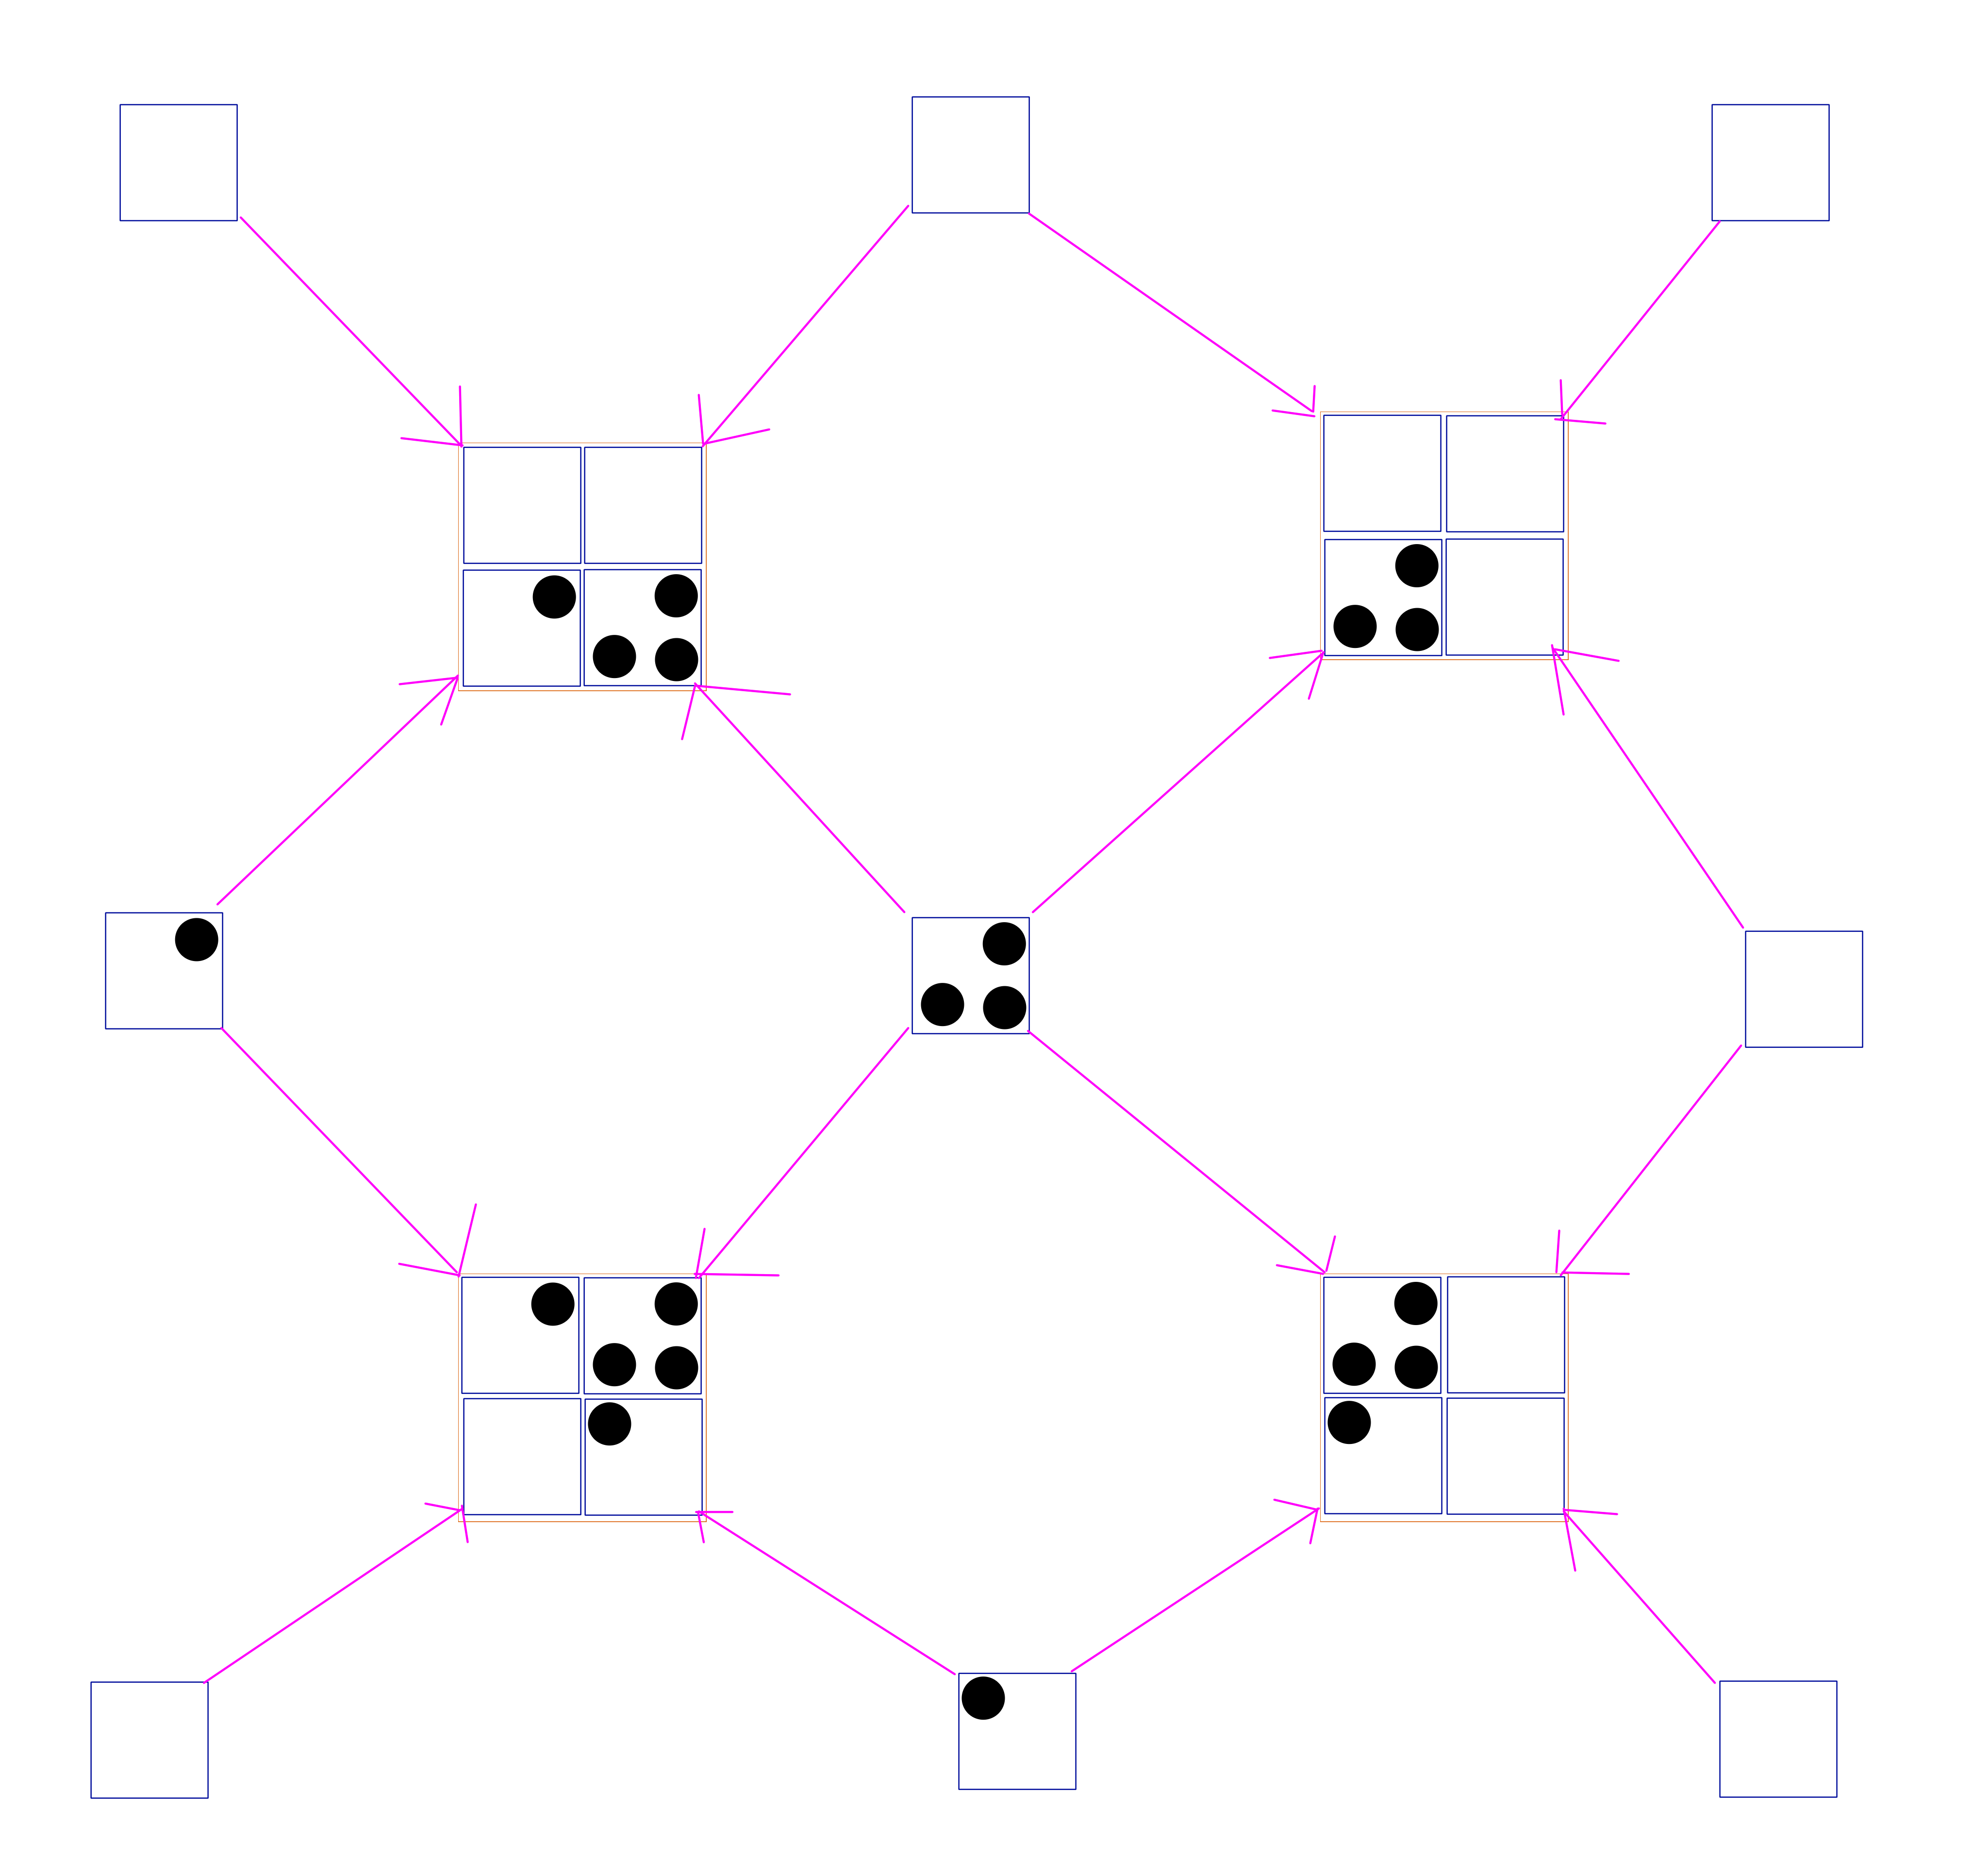
\includegraphics[scale=0.1]{images/imgHashlife/HashlifeStep3.png}
        \caption{Troisième étape de l'algorithme de Hashlife, ensuite on applique le même algorithme que almost hashlife sur les 4 nodes générées.}
\end{figure}
Pourtant un tel algorithme ne semble pas être bénéfique pour la performance car on calcule beaucoup de nodes déjà calculées, Cependant l'utilisation de la memoization va nous permettre d'exploiter ces propriétés sans trop affecter la durée entre deux changements de génération. Ainsi la première génération de Hashlife peux prendre beaucoup de temps a calculer (dans notre projet cela peux prendre entre 10 secondes et 5min dans le modele \textbf{metacellgalaxy.rle}), mais dès qu'assez de nodes ont été memoizées la performance devient difficile a représenter, alors que l'on calculait des dizaines de milliers de génération en une seconde avec almost-Hashlife on peut maintenant calculer si vite que le nombre de génération est difficile a retenir dans un entier long non-signé dont la limite est \textbf{18,446,744,073,709,551,615} , sans compter le fait qu'on peux augmenter la taille de l'arbre car plus l'arbre est gros plus on saute de générations! Il a donc été nécessaire d'imposer un court délai (\textit{5ms}) entre deux saut de génération de Hashlife afin que l'on puisse observer ce que fait l'algorithme. 

Ainsi Hashlife nous permet de simuler le jeu de la vie de la manière la plus rapide possible, que pouvons nous faire avec?

\subsection{résultats}
Voici une section un peux plus intéressante! Tout les modèles que nous allons vous montrer sont importés et simulés dans notre projet grâce a un lecteur RLE vous en trouverez plus d'informations dans la partie interface graphique. Tous ces modèles proviennent de \href{https://conwaylife.com/wiki/}{ce site}. Cessons donc parler d'algorithmes voyons voir se qu'ils ont dans le ventre:
\begin{figure}[H]
        \center
        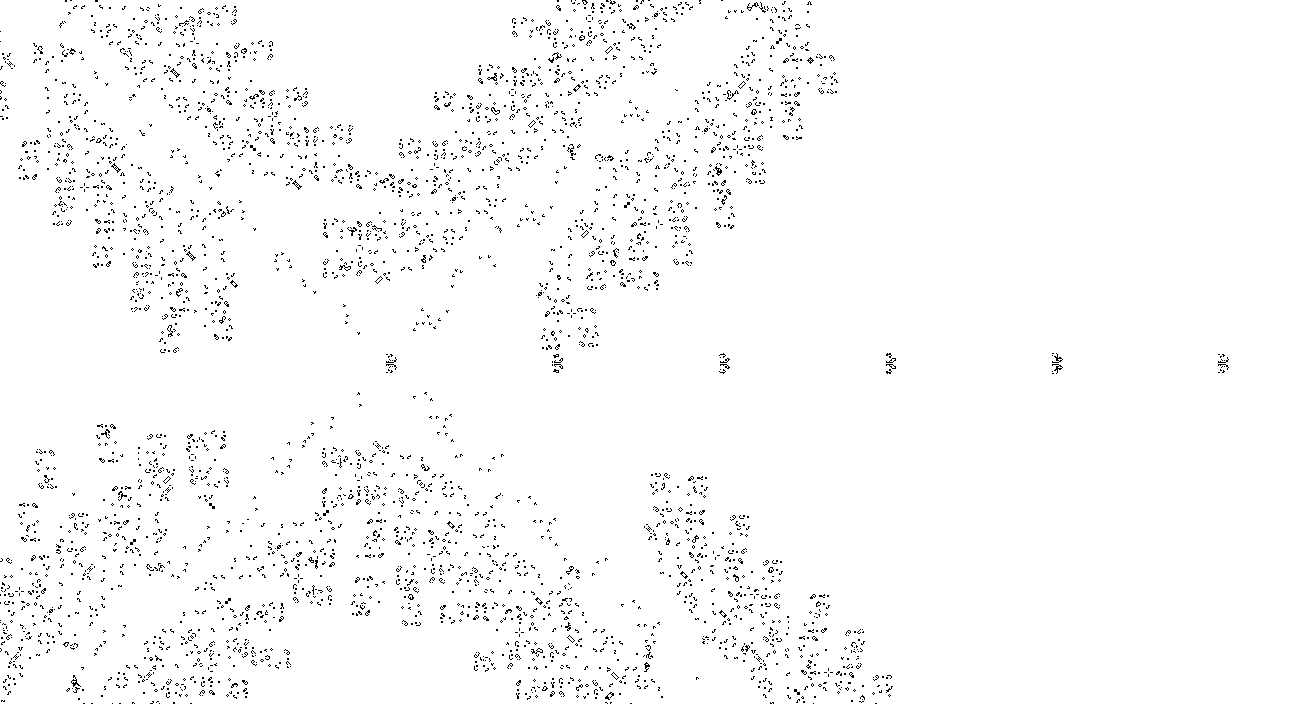
\includegraphics[scale=0.3]{images/imgHashlife/biggun.png}
        \caption{un pistolet a gros vaisseaux, almost hashlife suffit pour voir ce modele en action}
\end{figure}


\begin{figure}[H]
        \center
        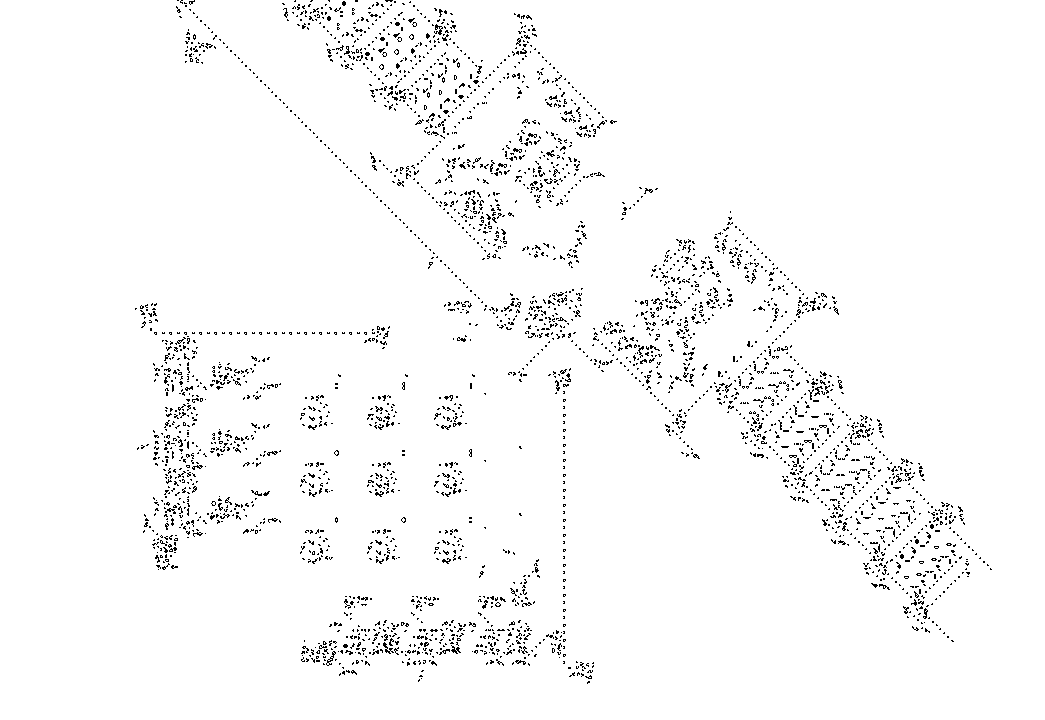
\includegraphics[scale=0.3]{images/imgHashlife/turingmachine.png}
        \caption{une machine de turing qui calcule les nombres premiers,
        on peux voir la sortie de celle ci en bas a gauche en flux de gliders}
\end{figure}

Les modèles suivants sont visionnables en temps réel grâce a hashlife

\begin{figure}[H]
        \center
        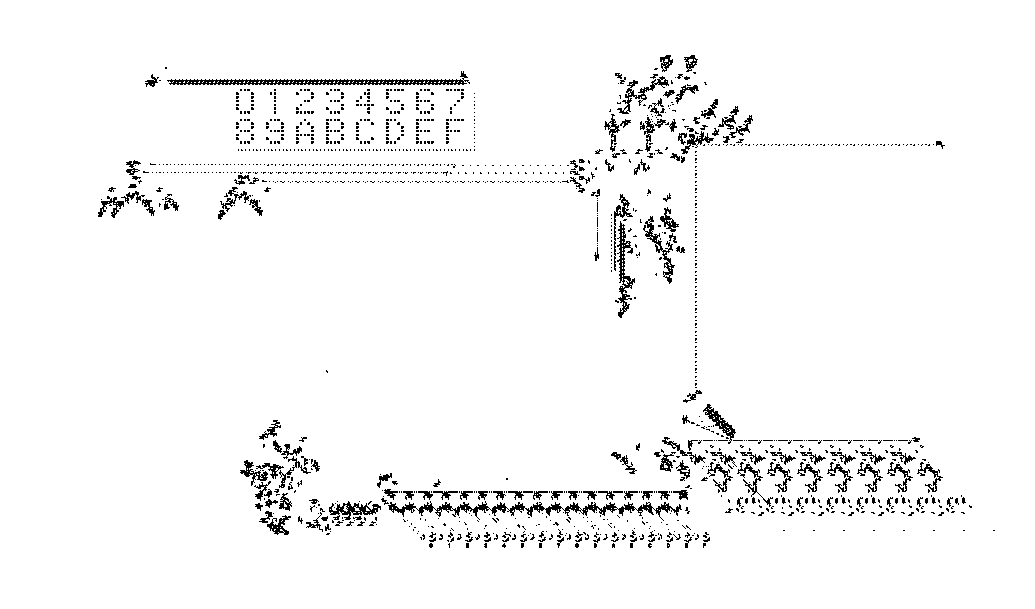
\includegraphics[scale=0.3]{images/imgHashlife/display.png}
        \caption{un affichage de lettres et chiffres on peux le voir afficher en temps réel chaque ligne de l'affichage. La première génération peux prendre \textit{45s}}
\end{figure}

\begin{figure}[H]
        \center
        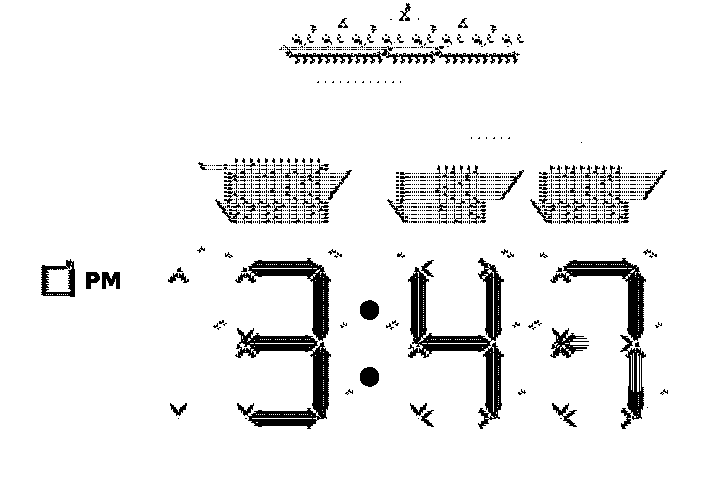
\includegraphics[scale=0.3]{images/imgHashlife/clock.png}
        \caption{une horloge digitale on peux la voir changer d'heure la première génération peux prendre \textit{1min20}}
\end{figure}

Et un dernier pour la route, et aussi le plus impressionnant!
\begin{figure}[H]
        \center
        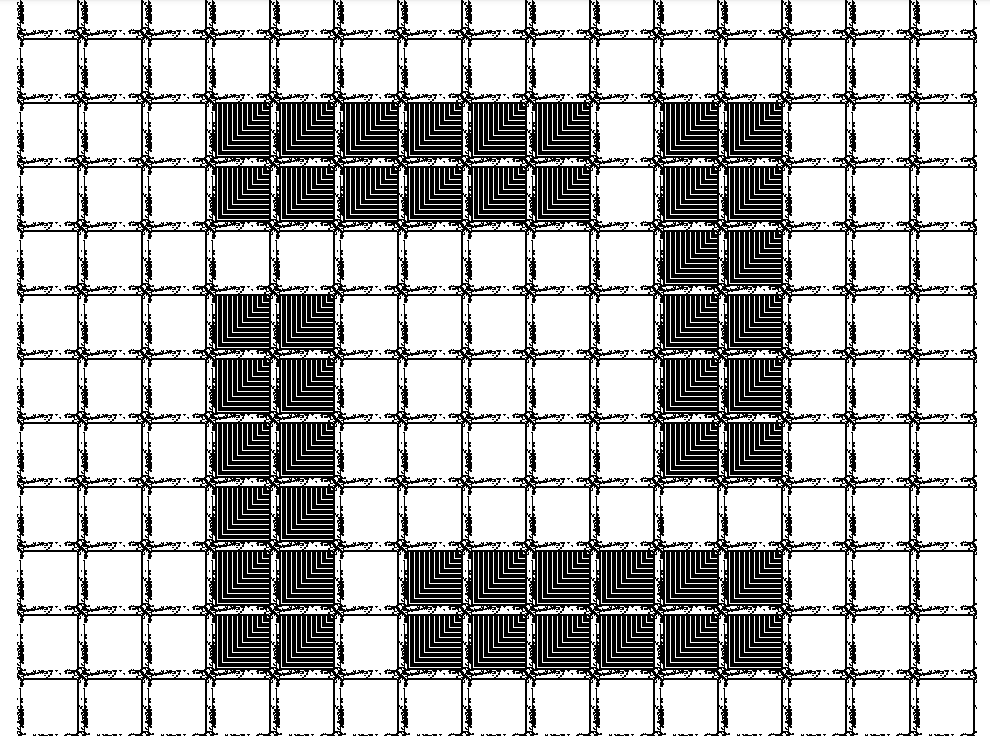
\includegraphics[scale=0.3]{images/imgHashlife/metacellgalaxy.png}
        \caption{le saint graal, le jeux de la vie dans le jeu de la vie grâce aux metacells, ici la galaxie de Kok la première génération peux prendre environ \textit{3-5min}, ce pattern est très dur a simuler sur mon petit laptop}
\end{figure}

Voila qui conclus cette explication de Hashlife.
